\documentclass[12pt,letterpaper]{article}
\usepackage[utf8]{inputenc}
\usepackage[T1]{fontenc}
\usepackage{lmodern}
\usepackage[spanish,es-tabla]{babel}
\addto\captionsspanish{\renewcommand{\contentsname}{\'{I}ndice}}
\usepackage[margin=1in,headheight=15pt]{geometry}
\usepackage{graphicx}
\usepackage{amsmath}
\usepackage{fancyhdr}
\usepackage{placeins}
\usepackage{float}
\usepackage{needspace}
\usepackage{array,tabularx}
\usepackage{enumitem}
\usepackage{microtype}
\usepackage{xurl}
\usepackage[hidelinks]{hyperref}
\hypersetup{pdftitle={Informe Laboratorio 3},pdfauthor={Matías Nicolás Primero Vigneau Andrades},pdfsubject={Criptografía: análisis del hash de contraseñas en MobileRead}}
\urlstyle{tt}
\setlength{\emergencystretch}{2em}
\setlength{\parindent}{1.5em}
\setlength{\parskip}{0pt}
\pagestyle{fancy}
\fancyhf{}
\fancyhead[L]{\small\nouppercase{\rightmark}}
\fancyfoot[C]{\thepage}
\renewcommand{\headrulewidth}{0.4pt}
\renewcommand{\sectionmark}[1]{}
\renewcommand{\subsectionmark}[1]{}
\makeatletter
\renewcommand{\@seccntformat}[1]{\csname the#1\endcsname.\quad}
\makeatother
\setcounter{tocdepth}{2}
\setlist[enumerate]{leftmargin=*,itemsep=0.8em}
\newcommand{\evidencia}[3]{%
 \begin{figure}[htbp]
  \centering
  \includegraphics[width=\linewidth,trim=0 60bp 0 96bp,clip]{figuras/#1}
  \caption{#2}\label{fig:#3}
 \end{figure}}
\title{Informe Laboratorio 3}
\author{\normalsize Sección 4\\[0.35em]
 \normalsize Alumno Matías Nicolás Primero Vigneau Andrades\\
 \normalsize e-mail: matias.vigneau@mail.udp.cl}
\date{\normalsize Octubre de 2026}
\begin{document}
\maketitle
\tableofcontents
\clearpage


\section{Descripción de actividades}
\markboth{1\quad Descripción de actividades}{1\quad Descripción de actividades}

Se analizó el tratamiento de contraseñas en el navegador de MobileRead Forums, disponible en \url{https://www.mobileread.com/forums/}. El objetivo fue identificar el hash utilizado en registro y acceso, reproducir el cálculo en la consola del navegador e intentar una autenticación sustituyendo los hashes de una contraseña incorrecta por los de la contraseña correcta.

La experiencia se realizó el 23 de octubre de 2026 sobre la cuenta propia \path|MatiasLab2326|. Se utilizó una contraseña exclusiva y temporal, \path|elmoyo123|, que se cambió al terminar. El entorno fue Linux, Chromium integrado en Burp Suite Community Edition 2026.9.2 y su proxy local. Se conservaron capturas originales y solicitudes completas en almacenamiento privado; las figuras del informe contienen recortes identificados y recuadros sobre los datos relevantes.

El procedimiento consistió en revisar el código público, crear y activar la cuenta, calcular los hashes, capturar un acceso correcto y cerrar la sesión. Luego se envió una contraseña incorrecta como control negativo. Finalmente, en una nueva solicitud se sustituyeron únicamente los dos campos MD5 y se comprobó el resultado en la respuesta y en el panel privado. La sesión se cerró antes de comenzar las pruebas para no confundir el acceso automático del registro con una autenticación obtenida mediante el hash.

\begin{table}[H]
\centering\small
\begin{tabularx}{\linewidth}{@{}>{\raggedright\arraybackslash}p{3cm}>{\raggedright\arraybackslash}p{2.4cm}>{\raggedright\arraybackslash}X>{\raggedright\arraybackslash}p{3.15cm}@{}}
\hline
Prueba & Entrada & Modificación en Burp & Resultado\\ \hline

Control positivo & \path|elmoyo123| & Ninguna & Acceso y panel privado\\[0.25em]

Control negativo & \path|elmoyo124| & Ninguna & Credenciales rechazadas\\[0.25em]

Sustitución & \path|elmoyo124| & Los dos hashes correctos & Acceso y panel privado\\[0.25em]

Cierre & Clave antigua & Ninguna & Credenciales rechazadas\\[0.25em]

\hline\end{tabularx}
\caption{Controles y prueba de sustitución realizados con la cuenta propia.}
\end{table}

Las pruebas se limitaron al cliente y al comportamiento de esta cuenta. No se inspeccionaron la base de datos, el código del servidor ni cuentas de terceros. Las políticas publicadas y las observaciones experimentales se presentan por separado.



\clearpage
\section{Desarrollo de actividades según criterio de rúbrica}
\markboth{2\quad Desarrollo de actividades según criterio de rúbrica}{2\quad Desarrollo de actividades según criterio de rúbrica}

\FloatBarrier
\subsection{Identifica el algoritmo hash utilizado para las contraseñas al momento del registro en el sitio web}
\markboth{2.1\quad Algoritmo hash en el registro}{2.1\quad Algoritmo hash en el registro}

Se abrió el formulario real de registro (Figura~\ref{fig:contexto-registro}) y se examinó su código fuente. El evento \path|onsubmit| llama a \path|verify_passwords(password, passwordconfirm)|. Esta función exige que ambas contraseñas estén presentes y coincidan; después invoca \path|md5hash| para completar \path|password_md5| y \path|passwordconfirm_md5|. La biblioteca cargada es \path|vbulletin_md5.js?v=385|, alojada en \url{https://www2.mobileread.com/c/} \cite{ref1,ref2}. La Figura~\ref{fig:1} conecta la biblioteca, las llamadas y el envío del formulario.

\begin{figure}[H]
 \centering
 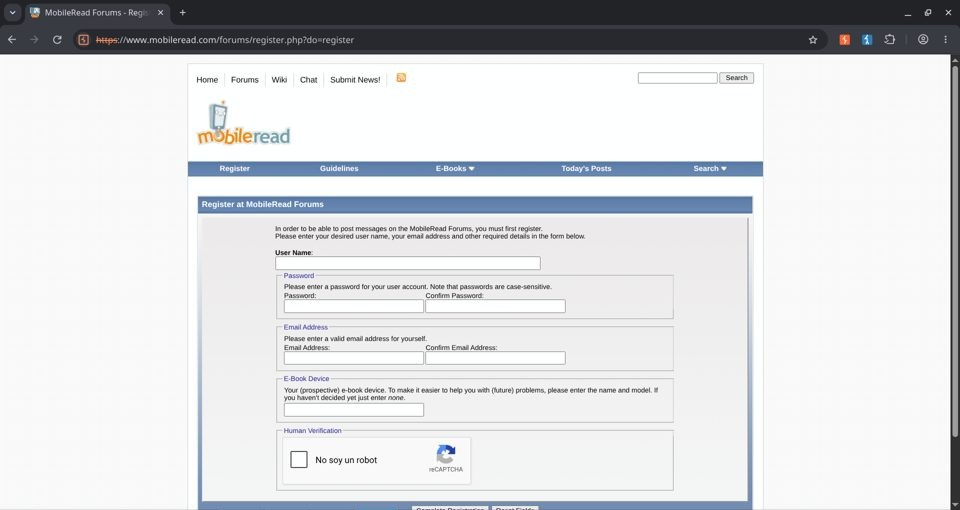
\includegraphics[width=0.78\linewidth]{figuras/contexto_registro.jpg}
 \caption{Vista general del formulario de registro de MobileRead utilizado al crear la cuenta de laboratorio.}
 \label{fig:contexto-registro}
\end{figure}

\evidencia{01_registro_codigo.png}{Registro: biblioteca, generación de hashes y evento que la invoca.}{1}

Se completó el registro de la cuenta propia y se interceptó el POST a \path|/forums/register.php?do=addmember| antes de reenviarlo. Los campos \path|password| y \path|passwordconfirm| estaban vacíos. En cambio, \path|password_md5| y \path|passwordconfirm_md5| contenían exactamente \path|02fa6c95e6f51a2e6cbb63fcf47adc5a|, valor que coincide con MD5 de la contraseña ASCII elegida. La Figura~\ref{fig:2} muestra los campos de la solicitud real. Después de reenviarla, el sitio confirmó el registro y envió el correo de activación; la activación se comprobó recargando la portada.

\evidencia{02_registro_peticion.png}{Registro interceptado: dos campos MD5 y contraseñas en texto plano vacías.}{2}

Por tanto, el algoritmo observado en el cliente durante el registro es MD5, con salida de 128 bits representada mediante 32 caracteres hexadecimales. La conclusión se basa en la implementación y en la solicitud, no únicamente en la longitud del valor. Esta evidencia no determina cómo almacena las contraseñas el servidor.

\FloatBarrier
\subsection{Identifica el algoritmo hash utilizado para las contraseñas al momento de iniciar sesión}
\markboth{2.2\quad Algoritmo hash en el inicio de sesión}{2.2\quad Algoritmo hash en el inicio de sesión}

En DevTools se consultó el formulario de acceso real del DOM y la representación de las funciones cargadas, mediante \path|outerHTML|, \path|md5hash.toString()| y \path|hex_md5.toString()|. El formulario usa POST a \path|login.php?do=login| y ejecuta \path|md5hash(vb_login_password, vb_login_md5password, vb_login_md5password_utf, 0)| al enviarse. En la Figura~\ref{fig:3} se señalan el evento y los fragmentos pertinentes de las funciones \cite{ref1,ref2}.

\evidencia{03_login_codigo.png}{Login: conexión del formulario con MD5 e implementación cargada en el navegador.}{3}

La función produce el campo principal con \path|hex_md5(str_to_ent(trim(B.value)))| y el alternativo con \path|hex_md5(trim(B.value))|. Cuando el cuarto argumento vale cero, vacía el campo de entrada. \path|hex_md5| llama a \path|core_md5|. Esto identifica MD5 también durante el acceso y explica por qué la solicitud real contiene hashes junto a un campo de contraseña vacío.

\path|trim| elimina espacios en blanco al principio y al final. \path|str_to_ent| transforma las unidades UTF-16 mayores que 255 en entidades numéricas. Por ello, el nombre del campo terminado en \path|_utf| no basta para afirmar que utiliza MD5 sobre UTF-8 estándar. Para \path|elmoyo123|, que solo contiene caracteres ASCII y carece de espacios extremos, las dos variantes coinciden con MD5 convencional. El script de verificación adicional reproduce cuatro casos locales, incluidos espacios extremos y un carácter mayor que 255; estas comprobaciones no sustituyen la prueba del navegador.

\FloatBarrier
\subsection{Genera el hash de la contraseña desde la consola del navegador}
\markboth{2.3\quad Hash desde la consola del navegador}{2.3\quad Hash desde la consola del navegador}

Con la página del foro cargada se ejecutó \path|scripts/hash_consola.js| en la consola. El script comprueba que existan \path|md5hash| y \path|hex_md5|, solicita la contraseña temporal y crea tres objetos con propiedad \path|value| para reproducir los argumentos de la función del sitio. No realiza solicitudes ni modifica el formulario. Devuelve los resultados para que DevTools los muestre, pues \path|console.table| no estaba disponible como función en esta página.

\evidencia{04_consola.png}{Ejecución real en DevTools: ambos campos producen el mismo hash de 32 caracteres.}{4}

La llamada central fue \path|md5hash(entrada, normal, utf, 0)|. Para \path|elmoyo123|, tanto \path|vb_login_md5password| como \path|vb_login_md5password_utf| produjeron \path|02fa6c95e6f51a2e6cbb63fcf47adc5a|. La Figura~\ref{fig:4} muestra la ejecución y el arreglo expandido. Se compararon los 32 caracteres de cada salida con sus campos correspondientes en la solicitud interceptada del punto 2.4; ambos coincidieron exactamente.

El archivo completo del script se incluye en el repositorio del anexo. La contraseña mostrada corresponde exclusivamente a la experiencia y dejó de ser válida después del cambio final; la nueva contraseña no forma parte del informe.

\FloatBarrier
\subsection{Intercepta el tráfico login con Burp Suite}
\markboth{2.4\quad Interceptación del login con Burp Suite}{2.4\quad Interceptación del login con Burp Suite}

Se cerró explícitamente la sesión inicial y el servidor mostró \texttt{All cookies cleared}. Luego se abrió el formulario de acceso, se mantuvo desmarcado \texttt{Remember Me} y se introdujeron el usuario propio y la contraseña correcta. Se activó la interceptación del proxy y se envió el formulario. En Burp se observó el POST a \path|/forums/login.php?do=login|, conservado antes de reenviarlo \cite{ref3}. La Figura~\ref{fig:contexto-burp} presenta el entorno de interceptación.

\begin{figure}[htbp]
 \centering
 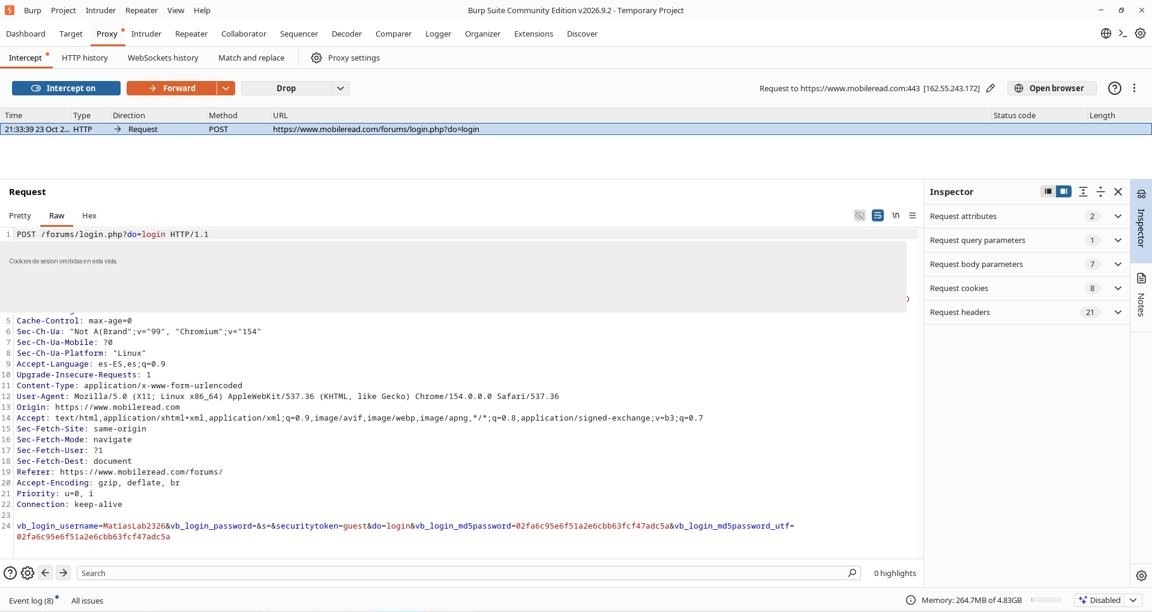
\includegraphics[width=0.93\linewidth]{figuras/contexto_burp.jpg}
 \caption{Vista general de Burp Suite durante la interceptación del tráfico de inicio de sesión.}
 \label{fig:contexto-burp}
\end{figure}


\evidencia{05_login_correcto_peticion.png}{Control positivo: solicitud real con usuario, contraseña vacía y los dos hashes correctos.}{5}

La solicitud contenía \path|vb_login_username=MatiasLab2326| y \path|vb_login_password| vacío. Los campos \path|vb_login_md5password| y \path|vb_login_md5password_utf| coincidieron con las salidas de la consola. Tras reenviar el POST y desactivar la interceptación, la respuesta indicó el acceso de \path|MatiasLab2326|. Se abrió además \path|/forums/usercp.php| y se comprobó que mostraba el panel privado y la identidad de la cuenta, como se observa en la Figura~\ref{fig:6}.

\evidencia{06_login_correcto_panel.png}{Acceso al panel privado después del login de control.}{6}

La respuesta HTTP fue \texttt{200 OK}, pero la autenticación se determinó por el contenido y el panel privado. Como se comprobó en el control negativo, el servidor también utiliza \texttt{200 OK} para un rechazo de credenciales; por sí solo, ese estado no prueba un acceso exitoso.

\FloatBarrier
\subsection{Realizar el intento de login por medio del hash}
\markboth{2.5\quad Intento de login por medio del hash}{2.5\quad Intento de login por medio del hash}

Primero se cerró la sesión del control positivo. Se introdujo \path|elmoyo124| como contraseña incorrecta y se interceptó el envío sin modificarlo. Los dos campos MD5 contenían \path|ae6b1f57beecb243ebf9df6179264ff3|, distinto del valor correcto. La Figura~\ref{fig:7} documenta esta solicitud.

\evidencia{07_login_incorrecto_peticion.png}{Control negativo: campos calculados a partir de elmoyo124.}{7}

Al reenviarla, el sitio rechazó el usuario o la contraseña. El mensaje indicó que se había utilizado un intento de cinco y que, al agotarlos, impediría el acceso durante quince minutos. Se conservó el aviso de la Figura~\ref{fig:8}, sin agotar los intentos ni comprobar experimentalmente el bloqueo.

\evidencia{08_login_incorrecto_resultado.png}{Rechazo real del control negativo y aviso del límite de intentos.}{8}

A continuación, todavía sin una sesión autenticada, se generó una nueva solicitud con \path|elmoyo124| y se retuvo en Burp. Se registró el estado anterior a la edición (Figura~\ref{fig:9}). En el editor de la petición se reemplazaron únicamente \path|vb_login_md5password| y \path|vb_login_md5password_utf| por \path|02fa6c95e6f51a2e6cbb63fcf47adc5a|, obtenido en el punto 2.3. Se conservaron el usuario, las cabeceras, el campo de texto plano vacío y los demás parámetros. La comparación local de ambas solicitudes confirmó que solo variaron esos dos campos. La Figura~\ref{fig:10} muestra el estado posterior a la sustitución.

\evidencia{09_sustitucion_antes.png}{Nueva solicitud generada con la contraseña incorrecta, antes de editarla.}{9}

\evidencia{10_sustitucion_despues.png}{Misma solicitud después de sustituir exclusivamente los dos campos MD5.}{10}

Se reenvió la solicitud modificada. La respuesta incluyó el saludo de autenticación para \path|MatiasLab2326| y Burp marcó la petición 750 como editada (Figura~\ref{fig:11}). Después se abrió nuevamente \path|/forums/usercp.php| y se obtuvo el panel privado de la cuenta (Figura~\ref{fig:12}). El cierre previo de sesión, el rechazo del control negativo y la ausencia de cookies \path|bbuserid| y \path|bbpassword| en la solicitud ayudan a separar este resultado de una autenticación previa. Había cookies de navegación y una sesión invitada; no se afirma ausencia de todas las cookies.

El resultado fue exitoso: el servidor aceptó el hash correcto aunque la nueva entrada del formulario hubiera sido incorrecta. En el alcance de esta experiencia, el valor enviado funciona como una credencial reutilizable. Se trata de la sustitución y reutilización solicitada por el laboratorio; no se encontró una colisión, no se invirtió MD5 y no se obtuvo una contraseña ajena. La prueba tampoco demuestra que cualquier solicitud pueda repetirse indefinidamente o desde cualquier contexto.

\evidencia{11_sustitucion_respuesta.png}{Respuesta a la petición modificada: saludo de autenticación para la cuenta propia.}{11}

\evidencia{12_sustitucion_panel.png}{Panel privado accesible después de la sustitución de hashes.}{12}



\FloatBarrier
\Needspace{15\baselineskip}
\subsection{Identifica las políticas de privacidad o seguridad}
\markboth{2.6\quad Políticas de privacidad y seguridad}{2.6\quad Políticas de privacidad y seguridad}

Se revisó la declaración de privacidad enlazada por el sitio: \url{https://www.mobileread.com/forums/faq.php?faq=vb_faq#faq_privacy_statement} \cite{ref4}. La política indica que el registro requiere usuario, contraseña y correo. Explica que las cookies permiten iniciar sesión y personalizar el servicio. La Figura~\ref{fig:13} muestra ambos fragmentos.

\evidencia{13_politica_registro.png}{Fragmentos de la política relacionados con registro y cookies de acceso.}{13}


\FloatBarrier
La sección Security declara medidas generales contra pérdida, uso indebido y alteración de información; recomienda proteger las credenciales y cambiar contraseña y correo desde el perfil si se sospecha un compromiso. El documento muestra como última actualización el 28 de noviembre de 2014, tal como se observa en la Figura~\ref{fig:14}.

\evidencia{14_politica_seguridad.png}{Declaración de seguridad y fecha de actualización publicada.}{14}


El texto consultado no especifica el algoritmo de almacenamiento, la sal, el coste de derivación ni un mecanismo concreto contra la reutilización del hash del cliente. La falta de esos detalles en la política no demuestra su ausencia en el servidor. La prueba del punto 2.5 sí aporta evidencia directa de que el valor correcto enviado por el navegador fue aceptado en una nueva solicitud modificada.
\FloatBarrier

\FloatBarrier
\Needspace{19\baselineskip}
\subsection{Comente 4 conclusiones sobre la seguridad del sitio escogido}
\markboth{2.7\quad Cuatro conclusiones sobre la seguridad}{2.7\quad Cuatro conclusiones sobre la seguridad}

\begin{enumerate}

\item El hash del cliente resultó reutilizable para autenticar la cuenta de prueba. El control con \path|elmoyo124| fue rechazado, mientras que una nueva solicitud con esa entrada y los dos hashes correctos permitió abrir el panel privado (Figuras~\ref{fig:7} a~\ref{fig:12}). Ocultar el texto plano en la solicitud no evita este resultado: quien obtenga el valor reutilizable podría utilizarlo como credencial en condiciones equivalentes a las ensayadas. La protección debe contemplar la exposición y reutilización de ese valor.

\item El uso de MD5 merece una revisión, pero la prueba realizada no explotó sus colisiones. El código y la consola mostraron una transformación rápida y determinista de la contraseña (Figuras~\ref{fig:1}, \ref{fig:3} y~\ref{fig:4}). RFC 6151 documenta debilidades de resistencia a colisiones de MD5 \cite{ref5}; aquí bastó reutilizar el hash conocido. Para almacenamiento, OWASP recomienda funciones adaptativas como Argon2id con sal \cite{ref6}. Esa recomendación se dirige al diseño del servidor: esta experiencia no observó su base de datos, y cambiar solo MD5 por otro hash determinista en el cliente no resuelve por sí mismo la reutilización demostrada.

\item HTTPS y el campo de texto plano vacío no eliminan el riesgo en los extremos de la comunicación. Las solicitudes al foro usaron HTTPS y el código vació el campo original (Figuras~\ref{fig:2} y~\ref{fig:5}). Burp pudo observar los valores porque el navegador estaba configurado expresamente para utilizar su proxy. Esto no prueba que un observador pasivo pueda leer HTTPS; demuestra que la confidencialidad del canal y la protección de la credencial en el cliente son problemas distintos. Una filtración del valor en un extremo seguiría siendo relevante por el resultado del punto 2.5.

\item Los controles observados tienen un alcance concreto. El sitio rechazó una contraseña incorrecta, anunció un límite de intentos y permitió cambiar la contraseña; después del cambio, la clave antigua fue rechazada (Figuras~\ref{fig:8} y~\ref{fig:15}). Son medidas útiles frente a intentos inválidos y para retirar una credencial expuesta, pero no impidieron el acceso cuando se suministró el hash correcto durante la prueba. El bloqueo anunciado no fue provocado y no se evaluó el comportamiento de otros factores de autenticación o de otras cuentas.

\end{enumerate}

\FloatBarrier
\section*{Conclusiones y comentarios}
\addcontentsline{toc}{section}{Conclusiones y comentarios}
\markboth{Conclusiones y comentarios}{Conclusiones y comentarios}

Se identificó MD5 en el registro y en el acceso, se reprodujeron los dos campos de login en la consola y se compararon con el tráfico real de Burp. El control negativo permitió distinguir un rechazo normal del resultado de sustituir los hashes. La solicitud modificada obtuvo una respuesta de autenticación y acceso al panel privado, por lo que el valor enviado actuó como credencial reutilizable en las condiciones ensayadas.

Al terminar, cambié personalmente la contraseña temporal. El POST de actualización respondió con una redirección al panel de usuario. Después se cerró la sesión y se realizó un único intento con la contraseña anterior: fue rechazado. La Figura~\ref{fig:15} documenta este cierre. La nueva contraseña no se incluyó en las capturas ni en los archivos.

\evidencia{15_cambio_clave.png}{Actualización de contraseña y rechazo posterior de la clave antigua.}{15}

El resultado se limita al flujo observado el 23 de octubre de 2026 y a la cuenta propia utilizada. No permite inferir ausencia de sal o de una derivación adicional en el servidor, ni afirmar una vulnerabilidad universal de todos sus mecanismos de autenticación. Las figuras omiten cookies, tokens y correo personal innecesarios; sus originales se conservan de forma privada.

\clearpage
\phantomsection
\addcontentsline{toc}{section}{Referencias}

\renewcommand{\refname}{Referencias}
\begin{thebibliography}{9}
\markboth{Referencias}{Referencias}


\bibitem{ref1} MobileRead Forums. Portada y formularios de registro y acceso. \url{https://www.mobileread.com/forums/} y \url{https://www.mobileread.com/forums/register.php}. Consulta: 23 de octubre de 2026.


\bibitem{ref2} MobileRead. Biblioteca JavaScript \path|vbulletin_md5.js?v=385|. \url{https://www2.mobileread.com/c/vbulletin_md5.js?v=385}. Consulta: 23 de octubre de 2026.


\bibitem{ref3} PortSwigger. Intercepting HTTP traffic with Burp Proxy. \url{https://portswigger.net/burp/documentation/desktop/getting-started/intercepting-http-traffic}. Consulta: 23 de octubre de 2026.


\bibitem{ref4} MobileRead. Privacy Statement. \url{https://www.mobileread.com/forums/faq.php?faq=vb_faq#faq_privacy_statement}. Actualización declarada: 28 de noviembre de 2014. Consulta: 23 de octubre de 2026.


\bibitem{ref5} Turner, S. y Chen, L. RFC 6151: Updated Security Considerations for the MD5 Message-Digest and the HMAC-MD5 Algorithms. Marzo de 2011. \url{https://www.rfc-editor.org/info/rfc6151/}.


\bibitem{ref6} OWASP. Password Storage Cheat Sheet. \url{https://cheatsheetseries.owasp.org/cheatsheets/Password_Storage_Cheat_Sheet.html}. Consulta: 23 de octubre de 2026.

\end{thebibliography}
\FloatBarrier
\section*{Anexo. Código y evidencias en GitHub}
\addcontentsline{toc}{section}{Anexo. Código y evidencias en GitHub}
\markboth{Anexo. Código y evidencias en GitHub}{Anexo. Código y evidencias en GitHub}

Repositorio: \url{https://github.com/vigneauuu/lab3-criptografia-mobileread}.

El repositorio contiene \path|scripts/hash_consola.js|, la verificación local adicional y las quince figuras utilizadas en el informe. El manifiesto relaciona cada figura con sus recortes y el SHA-256 del original. No se incluyen el tráfico completo, las cookies, los tokens, las credenciales vigentes. El enlace del repositorio también debe agregarse como comentario en la entrega, según las instrucciones del laboratorio.

\end{document}
